\documentclass[12pt]{article}
\usepackage{amssymb,amsmath,graphicx,float,tikz,pgfplots}
\usepackage{mathtools}
\pgfplotsset{compat=1.7}
\DeclarePairedDelimiter{\evdel}{\langle}{\rangle}

\newcommand{\Lagr}{\mathcal{L}}
\newcommand{\Ham}{\mathcal{H}}
\newcommand{\pd}[3]{\frac{\partial^{#3} {#1}}{\partial{#2}^{#3}}}

\begin{document}

\begin{figure}[htbp]
\begin{center}
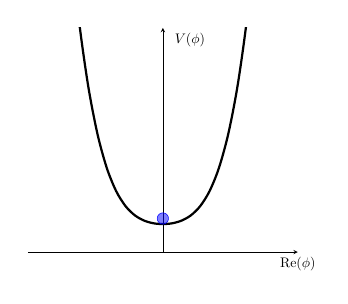
\begin{tikzpicture}[scale=0.5]
\begin{axis}[axis lines=middle, axis equal,
xtick=\empty,ytick=\empty,
xmin=-2,xmax=2,ymin=0,ymax=4,
x label style={at={(axis description cs:1.0,0.0)},anchor=north},
y label style={at={(axis description cs:0.6,1.0)},anchor=north},
xlabel={$\rm{Re}(\phi)$},ylabel={$V(\phi)$}]
\addplot[black, smooth, domain=-2:2, ultra thick] (x,0.5*x*x*x*x+0.5*x*x+0.5);
\addplot[blue, fill, fill opacity=0.5, smooth, domain=0:2*pi] ({0.1*cos(deg(x))},{0.1*sin(deg(x))+0.6});
\end{axis}
\end{tikzpicture}
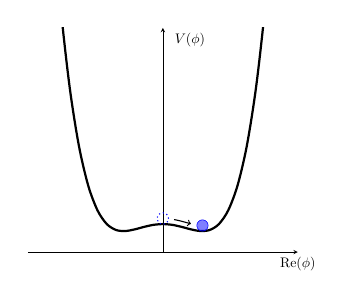
\begin{tikzpicture}[scale=0.5]
\begin{axis}[axis lines=middle, axis equal,
xtick=\empty,ytick=\empty,
xmin=-2,xmax=2,ymin=0,ymax=4,
x label style={at={(axis description cs:1.0,0.0)},anchor=north},
y label style={at={(axis description cs:0.6,1.0)},anchor=north},
xlabel={$\rm{Re}(\phi)$},ylabel={$V(\phi)$}]
\addplot[black, smooth, domain=-2:2, ultra thick] (x,0.5*x*x*x*x-0.5*x*x+0.5);
\addplot[->, black, smooth, domain=0.2:0.5, thick] (x,0.5*x*x*x*x-0.5*x*x+0.6);
\addplot[blue, dotted, thick, smooth, domain=0:2*pi] ({0.1*cos(deg(x))},{0.1*sin(deg(x))+0.6});
\addplot[blue, fill, fill opacity=0.5, smooth, domain=0:2*pi] ({0.1*cos(deg(x))+0.707},{0.1*sin(deg(x))+0.475});
\end{axis}
\end{tikzpicture}
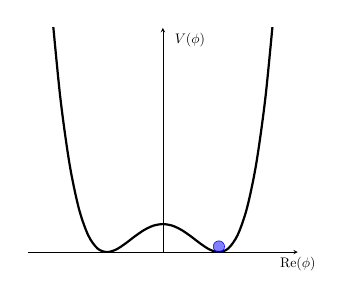
\begin{tikzpicture}[scale=0.5]
\begin{axis}[axis lines=middle, axis equal,
xtick=\empty,ytick=\empty,
xmin=-2,xmax=2,ymin=0,ymax=4,
x label style={at={(axis description cs:1.0,0.0)},anchor=north},
y label style={at={(axis description cs:0.6,1.0)},anchor=north},
xlabel={$\rm{Re}(\phi)$},ylabel={$V(\phi)$}]
\addplot[black, smooth, domain=-2:2, ultra thick] (x,0.5*x*x*x*x-1.0*x*x+0.5);
\addplot[blue, fill, fill opacity=0.5, smooth, domain=0:2*pi] ({0.1*cos(deg(x))+1.0},{0.1*sin(deg(x))+0.1});
\end{axis}
\end{tikzpicture}
\end{center}
\caption{Left: $E>0$, Right: $E<0$}
\label{fig:pr3PhaseSpace}
\end{figure}

\end{document}